\section{Results}
\subsection{Comparing integration techniques}

\begin{figure}
	\centering
	\includegraphics[width=1\linewidth, keepaspectratio]{tech_comp.eps}
	\caption{data techniques}
	\label{fig:tech-comp}
\end{figure}



\subsection{Comparing Batson correction}

\begin{figure}
	\centering
	\includegraphics[width=1\linewidth, keepaspectratio]{
		qmap_corr_comp.eps
		}
	\caption{Batson correction for qmap}
	\label{fig:bat-cor}
\end{figure}



\subsection{Interesting features from data}

\begin{figure}
	\centering
	\includegraphics[width=1\linewidth, keepaspectratio]{qmap_peak.eps}
	\caption{tracked peaks on stitched qmap}
	\label{fig:qmap-track}
\end{figure}


\begin{figure}
	\centering
	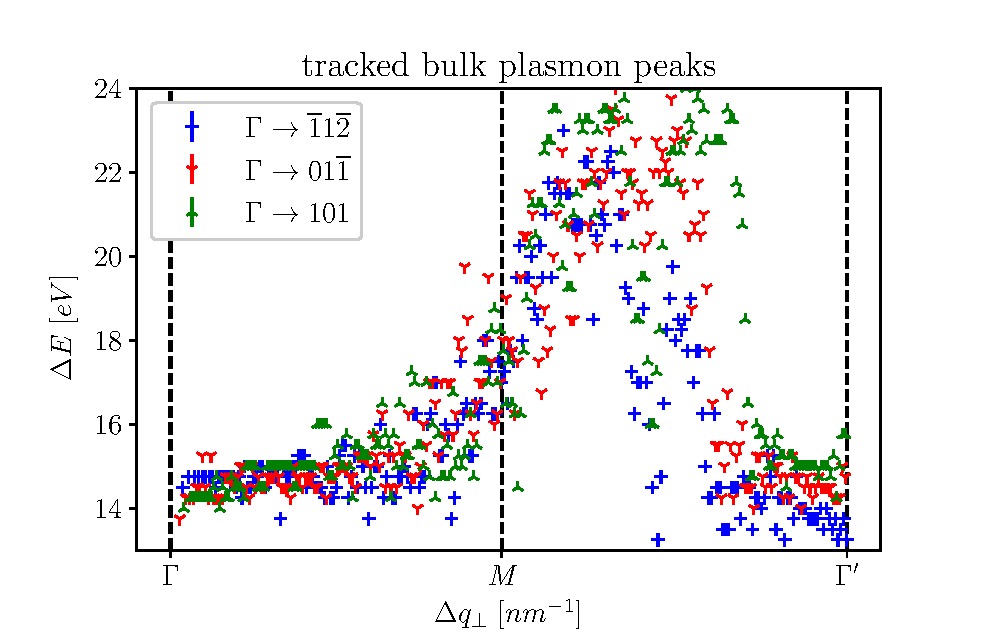
\includegraphics[width=0.5\linewidth, keepaspectratio]{plasmon_dispersion.eps}
	\caption{Tracked peaks of the plasmon dispersion.}
	\label{fig:plas_disp}
\end{figure}

\begin{figure}
	\centering
	\includegraphics[width=0.5\linewidth, keepaspectratio]{track_peak.eps}
	\caption{Tracked peaks of the plasmon dispersion.}
	\label{fig:track_peak}
\end{figure}